%\pagenumbering{arabic}

\section{Versões}

No mundo da computação, novos \textit{softwares} surgem quase todos os dias. Cada um desses \textit{softwares}, desde os mais simples até os mais avançados, passa por diversos processos e etapas de desenvolvimento, exigindo a criação de várias versões antes do lançamento. O versionamento é o processo de atribuir um nome ou uma numeração única para indicar o estado de um programa de computador \cite{wikipedia_versionamento}. De acordo com a mesma fonte, esses números geralmente seguem uma ordem crescente e refletem o desenvolvimento de melhorias ou correções de falhas do \textit{software}.

\begin{figure}
    \centering
    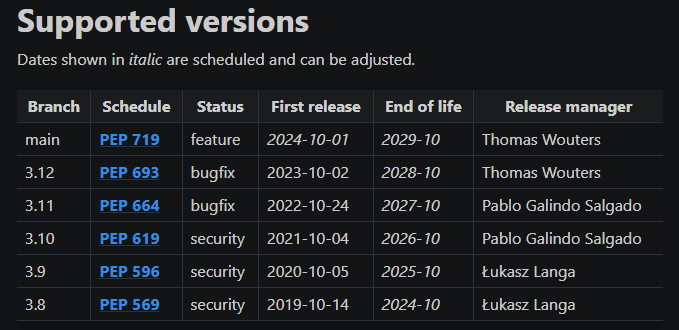
\includegraphics[width=0.5\linewidth]{Photos/Versoes-do-Python-4.png}
    \caption{Quadro de versões do \textit{Python} \cite{hashtagtreinamentos_python_versions}}
    \label{fig:enter-label}
\end{figure}

O \textit{Python} utiliza um esquema de versionamento conhecido como versionamento semântico \cite{hashtagtreinamentos_python_versions}, que é atualmente um dos sistemas de versionamento mais reconhecidos \cite{wikipedia_versionamento}. Esse esquema é composto por três números separados por pontos: MAJOR.MINOR.PATCH. O número MAJOR indica grandes mudanças que não são compatíveis com versões anteriores que possuem um número MAJOR diferente. O número MINOR é usado para adicionar funcionalidades compatíveis com a versão MAJOR atual. Já o número \textit{PATCH} refere-se a mudanças menores, como correções de \textit{bugs} e ajustes \cite{wikipedia_versionamento}.

No \textit{Python}, todas as versões possuem um status, que pode ser um dos seguintes: \textit{feature}, \textit{bugfix} ou \textit{security}. Quando uma versão está no status \textit{security}, significa que ela aceita apenas atualizações de segurança. Se uma versão está no status \textit{bugfix}, ela permite atualizações para correção de \textit{bugs} e também para segurança. Por último, o status \textit{feature} indica que a versão está aceitando atualizações que incluem novas funcionalidades \cite{hashtagtreinamentos_python_versions}.


\subsection{Versão 2.0}
A primeira versão significativa do \textit{Python} foi a 2.0, amplamente adotada pela comunidade de desenvolvedores. Ela trouxe recursos inovadores para a linguagem, como \textit{list comprehensions}, \textit{generators} e \textit{decorators} \cite{awari_python_version}.

\subsection{Versão 3.0}
Lançada em 2008, a versão 3.0 representa uma atualização significativa em relação à versão 2.0. Ela resolveu vários problemas e limitações da versão anterior, além de implementar diversas melhorias. As mudanças incluíram a eliminação da distinção entre strings e bytes, suporte nativo a Unicode e melhor gerenciamento de memória \cite{awari_python_version}.

\subsection{Versão 3.5}
Lançada em 2015, a versão 3.5 introduziu melhorias importantes, como a adição do operador de matriz de índice e um suporte aprimorado para \textit{await/async} \cite{awari_python_version}.

\subsection{Versão 3.8}
Lançado em 2019, o Python 3.8 trouxe várias novas funcionalidades e melhorias. Uma das principais adições foi a atribuição de expressões de linguagem, que permite atribuir valores a variáveis com base em expressões condicionais. Além disso, o Python 3.8 introduziu a possibilidade de usar o caractere de sublinhado como separador numérico para melhorar a legibilidade de números grandes \cite{awari_python_version}.